\documentclass[twoside]{book}

% Packages required by doxygen
\usepackage{calc}
\usepackage{doxygen}
\usepackage{graphicx}
\usepackage[utf8]{inputenc}
\usepackage{makeidx}
\usepackage{multicol}
\usepackage{multirow}
\usepackage{textcomp}
\usepackage[table]{xcolor}

% Font selection
\usepackage[T1]{fontenc}
\usepackage{mathptmx}
\usepackage[scaled=.90]{helvet}
\usepackage{courier}
\usepackage{amssymb}
\usepackage{sectsty}
\renewcommand{\familydefault}{\sfdefault}
\allsectionsfont{%
  \fontseries{bc}\selectfont%
  \color{darkgray}%
}
\renewcommand{\DoxyLabelFont}{%
  \fontseries{bc}\selectfont%
  \color{darkgray}%
}

% Page & text layout
\usepackage{geometry}
\geometry{%
  a4paper,%
  top=2.5cm,%
  bottom=2.5cm,%
  left=2.5cm,%
  right=2.5cm%
}
\tolerance=750
\hfuzz=15pt
\hbadness=750
\setlength{\emergencystretch}{15pt}
\setlength{\parindent}{0cm}
\setlength{\parskip}{0.2cm}
\makeatletter
\renewcommand{\paragraph}{%
  \@startsection{paragraph}{4}{0ex}{-1.0ex}{1.0ex}{%
    \normalfont\normalsize\bfseries\SS@parafont%
  }%
}
\renewcommand{\subparagraph}{%
  \@startsection{subparagraph}{5}{0ex}{-1.0ex}{1.0ex}{%
    \normalfont\normalsize\bfseries\SS@subparafont%
  }%
}
\makeatother

% Headers & footers
\usepackage{fancyhdr}
\pagestyle{fancyplain}
\fancyhead[LE]{\fancyplain{}{\bfseries\thepage}}
\fancyhead[CE]{\fancyplain{}{}}
\fancyhead[RE]{\fancyplain{}{\bfseries\leftmark}}
\fancyhead[LO]{\fancyplain{}{\bfseries\rightmark}}
\fancyhead[CO]{\fancyplain{}{}}
\fancyhead[RO]{\fancyplain{}{\bfseries\thepage}}
\fancyfoot[LE]{\fancyplain{}{}}
\fancyfoot[CE]{\fancyplain{}{}}
\fancyfoot[RE]{\fancyplain{}{\bfseries\scriptsize Generated on Tue Sep 29 2015 23\-:22\-:11 for My Project by Doxygen }}
\fancyfoot[LO]{\fancyplain{}{\bfseries\scriptsize Generated on Tue Sep 29 2015 23\-:22\-:11 for My Project by Doxygen }}
\fancyfoot[CO]{\fancyplain{}{}}
\fancyfoot[RO]{\fancyplain{}{}}
\renewcommand{\footrulewidth}{0.4pt}
\renewcommand{\chaptermark}[1]{%
  \markboth{#1}{}%
}
\renewcommand{\sectionmark}[1]{%
  \markright{\thesection\ #1}%
}

% Indices & bibliography
\usepackage{natbib}
\usepackage[titles]{tocloft}
\setcounter{tocdepth}{3}
\setcounter{secnumdepth}{5}
\makeindex

% Hyperlinks (required, but should be loaded last)
\usepackage{ifpdf}
\ifpdf
  \usepackage[pdftex,pagebackref=true]{hyperref}
\else
  \usepackage[ps2pdf,pagebackref=true]{hyperref}
\fi
\hypersetup{%
  colorlinks=true,%
  linkcolor=blue,%
  citecolor=blue,%
  unicode%
}

% Custom commands
\newcommand{\clearemptydoublepage}{%
  \newpage{\pagestyle{empty}\cleardoublepage}%
}


%===== C O N T E N T S =====

\begin{document}

% Titlepage & ToC
\hypersetup{pageanchor=false}
\pagenumbering{roman}
\begin{titlepage}
\vspace*{7cm}
\begin{center}%
{\Large My Project }\\
\vspace*{1cm}
{\large Generated by Doxygen 1.8.6}\\
\vspace*{0.5cm}
{\small Tue Sep 29 2015 23:22:11}\\
\end{center}
\end{titlepage}
\clearemptydoublepage
\tableofcontents
\clearemptydoublepage
\pagenumbering{arabic}
\hypersetup{pageanchor=true}

%--- Begin generated contents ---
\chapter{Namespace Index}
\section{Namespace List}
Here is a list of all namespaces with brief descriptions\-:\begin{DoxyCompactList}
\item\contentsline{section}{\hyperlink{namespacevideorentalsystem}{videorentalsystem} }{\pageref{namespacevideorentalsystem}}{}
\end{DoxyCompactList}

\chapter{Hierarchical Index}
\section{Class Hierarchy}
This inheritance list is sorted roughly, but not completely, alphabetically\-:\begin{DoxyCompactList}
\item \contentsline{section}{carcruisecontrolsystem.\-Car\-Cruise\-Control\-System}{\pageref{classcarcruisecontrolsystem_1_1CarCruiseControlSystem}}{}
\item J\-Frame\begin{DoxyCompactList}
\item \contentsline{section}{carcruisecontrolsystem.\-Control}{\pageref{classcarcruisecontrolsystem_1_1Control}}{}
\item \contentsline{section}{carcruisecontrolsystem.\-Greeter}{\pageref{classcarcruisecontrolsystem_1_1Greeter}}{}
\end{DoxyCompactList}
\end{DoxyCompactList}

\chapter{Class Index}
\section{Class List}
Here are the classes, structs, unions and interfaces with brief descriptions\-:\begin{DoxyCompactList}
\item\contentsline{section}{\hyperlink{classcarcruisecontrolsystem_1_1CarCruiseControlSystem}{carcruisecontrolsystem.\-Car\-Cruise\-Control\-System} }{\pageref{classcarcruisecontrolsystem_1_1CarCruiseControlSystem}}{}
\item\contentsline{section}{\hyperlink{classcarcruisecontrolsystem_1_1Control}{carcruisecontrolsystem.\-Control} }{\pageref{classcarcruisecontrolsystem_1_1Control}}{}
\item\contentsline{section}{\hyperlink{classcarcruisecontrolsystem_1_1Greeter}{carcruisecontrolsystem.\-Greeter} }{\pageref{classcarcruisecontrolsystem_1_1Greeter}}{}
\end{DoxyCompactList}

\chapter{File Index}
\section{File List}
Here is a list of all files with brief descriptions\-:\begin{DoxyCompactList}
\item\contentsline{section}{\hyperlink{CostData_8java}{Cost\-Data.\-java} }{\pageref{CostData_8java}}{}
\item\contentsline{section}{\hyperlink{Costumer_8java}{Costumer.\-java} }{\pageref{Costumer_8java}}{}
\item\contentsline{section}{\hyperlink{CostumerForm_8java}{Costumer\-Form.\-java} }{\pageref{CostumerForm_8java}}{}
\item\contentsline{section}{\hyperlink{Movie_8java}{Movie.\-java} }{\pageref{Movie_8java}}{}
\item\contentsline{section}{\hyperlink{Producer_8java}{Producer.\-java} }{\pageref{Producer_8java}}{}
\item\contentsline{section}{\hyperlink{Rental_8java}{Rental.\-java} }{\pageref{Rental_8java}}{}
\item\contentsline{section}{\hyperlink{RentVideo_8java}{Rent\-Video.\-java} }{\pageref{RentVideo_8java}}{}
\item\contentsline{section}{\hyperlink{VideoData_8java}{Video\-Data.\-java} }{\pageref{VideoData_8java}}{}
\item\contentsline{section}{\hyperlink{VideoForm_8java}{Video\-Form.\-java} }{\pageref{VideoForm_8java}}{}
\item\contentsline{section}{\hyperlink{VideoRentalSystem_8java}{Video\-Rental\-System.\-java} }{\pageref{VideoRentalSystem_8java}}{}
\item\contentsline{section}{\hyperlink{Welcome_8java}{Welcome.\-java} }{\pageref{Welcome_8java}}{}
\end{DoxyCompactList}

\chapter{Namespace Documentation}
\hypertarget{namespacevideorentalsystem}{\section{Package videorentalsystem}
\label{namespacevideorentalsystem}\index{videorentalsystem@{videorentalsystem}}
}
\subsection*{Classes}
\begin{DoxyCompactItemize}
\item 
class \hyperlink{classvideorentalsystem_1_1CostData}{Cost\-Data}
\item 
class \hyperlink{classvideorentalsystem_1_1Costumer}{Costumer}
\item 
class \hyperlink{classvideorentalsystem_1_1CostumerForm}{Costumer\-Form}
\item 
class \hyperlink{classvideorentalsystem_1_1Movie}{Movie}
\item 
class \hyperlink{classvideorentalsystem_1_1Producer}{Producer}
\item 
class \hyperlink{classvideorentalsystem_1_1Rental}{Rental}
\item 
class \hyperlink{classvideorentalsystem_1_1RentVideo}{Rent\-Video}
\item 
class \hyperlink{classvideorentalsystem_1_1VideoData}{Video\-Data}
\item 
class \hyperlink{classvideorentalsystem_1_1VideoForm}{Video\-Form}
\item 
class \hyperlink{classvideorentalsystem_1_1VideoRentalSystem}{Video\-Rental\-System}
\item 
class \hyperlink{classvideorentalsystem_1_1Welcome}{Welcome}
\end{DoxyCompactItemize}

\chapter{Class Documentation}
\hypertarget{classvideorentalsystem_1_1CostData}{\section{videorentalsystem.\-Cost\-Data Class Reference}
\label{classvideorentalsystem_1_1CostData}\index{videorentalsystem.\-Cost\-Data@{videorentalsystem.\-Cost\-Data}}
}


Collaboration diagram for videorentalsystem.\-Cost\-Data\-:
\nopagebreak
\begin{figure}[H]
\begin{center}
\leavevmode
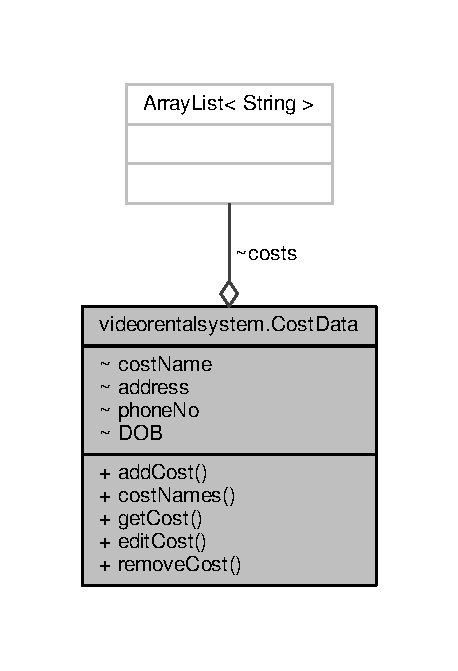
\includegraphics[width=220pt]{classvideorentalsystem_1_1CostData__coll__graph}
\end{center}
\end{figure}
\subsection*{Public Member Functions}
\begin{DoxyCompactItemize}
\item 
void \hyperlink{classvideorentalsystem_1_1CostData_a068ae4d12622331a36534360df8fa97d}{add\-Cost} (String cost\-Name, String address, String phone\-No, String D\-O\-B)
\item 
Array\-List$<$ String $>$ \hyperlink{classvideorentalsystem_1_1CostData_a49e580015e08b9dfe17f3d543717e68c}{cost\-Names} ()
\item 
void \hyperlink{classvideorentalsystem_1_1CostData_adec7aa3b57456c1962d4aa7f57741aef}{get\-Cost} (String cost\-Name)
\item 
void \hyperlink{classvideorentalsystem_1_1CostData_adaf884d21edc1c23d691f09c12f1ec2b}{edit\-Cost} (String oldcost\-Name, String newcost\-Name, String phone\-No, String address, String D\-O\-B)
\item 
void \hyperlink{classvideorentalsystem_1_1CostData_adcbc8c344fa0b7f1a6f2d0e428e65f6b}{remove\-Cost} (String cost\-Name)
\end{DoxyCompactItemize}


\subsection{Detailed Description}
\begin{DoxyAuthor}{Author}
abhinav 
\end{DoxyAuthor}


\subsection{Member Function Documentation}
\hypertarget{classvideorentalsystem_1_1CostData_a068ae4d12622331a36534360df8fa97d}{\index{videorentalsystem\-::\-Cost\-Data@{videorentalsystem\-::\-Cost\-Data}!add\-Cost@{add\-Cost}}
\index{add\-Cost@{add\-Cost}!videorentalsystem::CostData@{videorentalsystem\-::\-Cost\-Data}}
\subsubsection[{add\-Cost}]{\setlength{\rightskip}{0pt plus 5cm}void videorentalsystem.\-Cost\-Data.\-add\-Cost (
\begin{DoxyParamCaption}
\item[{String}]{cost\-Name, }
\item[{String}]{address, }
\item[{String}]{phone\-No, }
\item[{String}]{D\-O\-B}
\end{DoxyParamCaption}
)\hspace{0.3cm}{\ttfamily [inline]}}}\label{classvideorentalsystem_1_1CostData_a068ae4d12622331a36534360df8fa97d}
\hypertarget{classvideorentalsystem_1_1CostData_a49e580015e08b9dfe17f3d543717e68c}{\index{videorentalsystem\-::\-Cost\-Data@{videorentalsystem\-::\-Cost\-Data}!cost\-Names@{cost\-Names}}
\index{cost\-Names@{cost\-Names}!videorentalsystem::CostData@{videorentalsystem\-::\-Cost\-Data}}
\subsubsection[{cost\-Names}]{\setlength{\rightskip}{0pt plus 5cm}Array\-List$<$String$>$ videorentalsystem.\-Cost\-Data.\-cost\-Names (
\begin{DoxyParamCaption}
{}
\end{DoxyParamCaption}
)\hspace{0.3cm}{\ttfamily [inline]}}}\label{classvideorentalsystem_1_1CostData_a49e580015e08b9dfe17f3d543717e68c}
\hypertarget{classvideorentalsystem_1_1CostData_adaf884d21edc1c23d691f09c12f1ec2b}{\index{videorentalsystem\-::\-Cost\-Data@{videorentalsystem\-::\-Cost\-Data}!edit\-Cost@{edit\-Cost}}
\index{edit\-Cost@{edit\-Cost}!videorentalsystem::CostData@{videorentalsystem\-::\-Cost\-Data}}
\subsubsection[{edit\-Cost}]{\setlength{\rightskip}{0pt plus 5cm}void videorentalsystem.\-Cost\-Data.\-edit\-Cost (
\begin{DoxyParamCaption}
\item[{String}]{oldcost\-Name, }
\item[{String}]{newcost\-Name, }
\item[{String}]{phone\-No, }
\item[{String}]{address, }
\item[{String}]{D\-O\-B}
\end{DoxyParamCaption}
)\hspace{0.3cm}{\ttfamily [inline]}}}\label{classvideorentalsystem_1_1CostData_adaf884d21edc1c23d691f09c12f1ec2b}
\hypertarget{classvideorentalsystem_1_1CostData_adec7aa3b57456c1962d4aa7f57741aef}{\index{videorentalsystem\-::\-Cost\-Data@{videorentalsystem\-::\-Cost\-Data}!get\-Cost@{get\-Cost}}
\index{get\-Cost@{get\-Cost}!videorentalsystem::CostData@{videorentalsystem\-::\-Cost\-Data}}
\subsubsection[{get\-Cost}]{\setlength{\rightskip}{0pt plus 5cm}void videorentalsystem.\-Cost\-Data.\-get\-Cost (
\begin{DoxyParamCaption}
\item[{String}]{cost\-Name}
\end{DoxyParamCaption}
)\hspace{0.3cm}{\ttfamily [inline]}}}\label{classvideorentalsystem_1_1CostData_adec7aa3b57456c1962d4aa7f57741aef}
\hypertarget{classvideorentalsystem_1_1CostData_adcbc8c344fa0b7f1a6f2d0e428e65f6b}{\index{videorentalsystem\-::\-Cost\-Data@{videorentalsystem\-::\-Cost\-Data}!remove\-Cost@{remove\-Cost}}
\index{remove\-Cost@{remove\-Cost}!videorentalsystem::CostData@{videorentalsystem\-::\-Cost\-Data}}
\subsubsection[{remove\-Cost}]{\setlength{\rightskip}{0pt plus 5cm}void videorentalsystem.\-Cost\-Data.\-remove\-Cost (
\begin{DoxyParamCaption}
\item[{String}]{cost\-Name}
\end{DoxyParamCaption}
)\hspace{0.3cm}{\ttfamily [inline]}}}\label{classvideorentalsystem_1_1CostData_adcbc8c344fa0b7f1a6f2d0e428e65f6b}


The documentation for this class was generated from the following file\-:\begin{DoxyCompactItemize}
\item 
\hyperlink{CostData_8java}{Cost\-Data.\-java}\end{DoxyCompactItemize}

\hypertarget{classvideorentalsystem_1_1Costumer}{\section{videorentalsystem.\-Costumer Class Reference}
\label{classvideorentalsystem_1_1Costumer}\index{videorentalsystem.\-Costumer@{videorentalsystem.\-Costumer}}
}


Collaboration diagram for videorentalsystem.\-Costumer\-:
\nopagebreak
\begin{figure}[H]
\begin{center}
\leavevmode
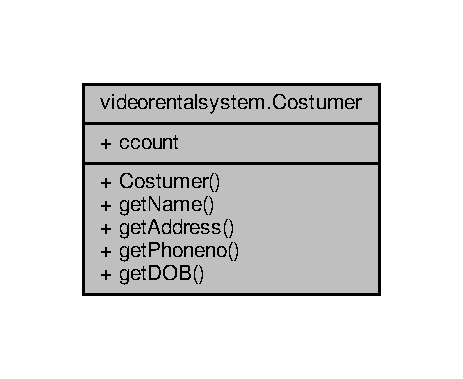
\includegraphics[width=222pt]{classvideorentalsystem_1_1Costumer__coll__graph}
\end{center}
\end{figure}
\subsection*{Public Member Functions}
\begin{DoxyCompactItemize}
\item 
\hyperlink{classvideorentalsystem_1_1Costumer_ab14784dcbcc0666a52028443cd5f8b4b}{Costumer} (String fname, String lname, String addr, String pno, String dob)
\item 
String \hyperlink{classvideorentalsystem_1_1Costumer_a7b5e9acd8cc041d5a41e8a6c5ae37b4c}{get\-Name} ()
\item 
String \hyperlink{classvideorentalsystem_1_1Costumer_af7955a56dc3398d6a7a1070b9a662f12}{get\-Address} ()
\item 
String \hyperlink{classvideorentalsystem_1_1Costumer_a21333c82e17dbfa6bab0dc41c343b356}{get\-Phoneno} ()
\item 
String \hyperlink{classvideorentalsystem_1_1Costumer_a7eb6bb7a7bf8601be08c336023d54bd3}{get\-D\-O\-B} ()
\end{DoxyCompactItemize}
\subsection*{Static Public Attributes}
\begin{DoxyCompactItemize}
\item 
static int \hyperlink{classvideorentalsystem_1_1Costumer_a8f4a5d4db773d971fad7a717a964f2ad}{ccount} =0
\end{DoxyCompactItemize}


\subsection{Detailed Description}
\begin{DoxyAuthor}{Author}
user 
\end{DoxyAuthor}


\subsection{Constructor \& Destructor Documentation}
\hypertarget{classvideorentalsystem_1_1Costumer_ab14784dcbcc0666a52028443cd5f8b4b}{\index{videorentalsystem\-::\-Costumer@{videorentalsystem\-::\-Costumer}!Costumer@{Costumer}}
\index{Costumer@{Costumer}!videorentalsystem::Costumer@{videorentalsystem\-::\-Costumer}}
\subsubsection[{Costumer}]{\setlength{\rightskip}{0pt plus 5cm}videorentalsystem.\-Costumer.\-Costumer (
\begin{DoxyParamCaption}
\item[{String}]{fname, }
\item[{String}]{lname, }
\item[{String}]{addr, }
\item[{String}]{pno, }
\item[{String}]{dob}
\end{DoxyParamCaption}
)\hspace{0.3cm}{\ttfamily [inline]}}}\label{classvideorentalsystem_1_1Costumer_ab14784dcbcc0666a52028443cd5f8b4b}


\subsection{Member Function Documentation}
\hypertarget{classvideorentalsystem_1_1Costumer_af7955a56dc3398d6a7a1070b9a662f12}{\index{videorentalsystem\-::\-Costumer@{videorentalsystem\-::\-Costumer}!get\-Address@{get\-Address}}
\index{get\-Address@{get\-Address}!videorentalsystem::Costumer@{videorentalsystem\-::\-Costumer}}
\subsubsection[{get\-Address}]{\setlength{\rightskip}{0pt plus 5cm}String videorentalsystem.\-Costumer.\-get\-Address (
\begin{DoxyParamCaption}
{}
\end{DoxyParamCaption}
)\hspace{0.3cm}{\ttfamily [inline]}}}\label{classvideorentalsystem_1_1Costumer_af7955a56dc3398d6a7a1070b9a662f12}
\hypertarget{classvideorentalsystem_1_1Costumer_a7eb6bb7a7bf8601be08c336023d54bd3}{\index{videorentalsystem\-::\-Costumer@{videorentalsystem\-::\-Costumer}!get\-D\-O\-B@{get\-D\-O\-B}}
\index{get\-D\-O\-B@{get\-D\-O\-B}!videorentalsystem::Costumer@{videorentalsystem\-::\-Costumer}}
\subsubsection[{get\-D\-O\-B}]{\setlength{\rightskip}{0pt plus 5cm}String videorentalsystem.\-Costumer.\-get\-D\-O\-B (
\begin{DoxyParamCaption}
{}
\end{DoxyParamCaption}
)\hspace{0.3cm}{\ttfamily [inline]}}}\label{classvideorentalsystem_1_1Costumer_a7eb6bb7a7bf8601be08c336023d54bd3}
\hypertarget{classvideorentalsystem_1_1Costumer_a7b5e9acd8cc041d5a41e8a6c5ae37b4c}{\index{videorentalsystem\-::\-Costumer@{videorentalsystem\-::\-Costumer}!get\-Name@{get\-Name}}
\index{get\-Name@{get\-Name}!videorentalsystem::Costumer@{videorentalsystem\-::\-Costumer}}
\subsubsection[{get\-Name}]{\setlength{\rightskip}{0pt plus 5cm}String videorentalsystem.\-Costumer.\-get\-Name (
\begin{DoxyParamCaption}
{}
\end{DoxyParamCaption}
)\hspace{0.3cm}{\ttfamily [inline]}}}\label{classvideorentalsystem_1_1Costumer_a7b5e9acd8cc041d5a41e8a6c5ae37b4c}
\hypertarget{classvideorentalsystem_1_1Costumer_a21333c82e17dbfa6bab0dc41c343b356}{\index{videorentalsystem\-::\-Costumer@{videorentalsystem\-::\-Costumer}!get\-Phoneno@{get\-Phoneno}}
\index{get\-Phoneno@{get\-Phoneno}!videorentalsystem::Costumer@{videorentalsystem\-::\-Costumer}}
\subsubsection[{get\-Phoneno}]{\setlength{\rightskip}{0pt plus 5cm}String videorentalsystem.\-Costumer.\-get\-Phoneno (
\begin{DoxyParamCaption}
{}
\end{DoxyParamCaption}
)\hspace{0.3cm}{\ttfamily [inline]}}}\label{classvideorentalsystem_1_1Costumer_a21333c82e17dbfa6bab0dc41c343b356}


\subsection{Member Data Documentation}
\hypertarget{classvideorentalsystem_1_1Costumer_a8f4a5d4db773d971fad7a717a964f2ad}{\index{videorentalsystem\-::\-Costumer@{videorentalsystem\-::\-Costumer}!ccount@{ccount}}
\index{ccount@{ccount}!videorentalsystem::Costumer@{videorentalsystem\-::\-Costumer}}
\subsubsection[{ccount}]{\setlength{\rightskip}{0pt plus 5cm}int videorentalsystem.\-Costumer.\-ccount =0\hspace{0.3cm}{\ttfamily [static]}}}\label{classvideorentalsystem_1_1Costumer_a8f4a5d4db773d971fad7a717a964f2ad}


The documentation for this class was generated from the following file\-:\begin{DoxyCompactItemize}
\item 
\hyperlink{Costumer_8java}{Costumer.\-java}\end{DoxyCompactItemize}

\hypertarget{classvideorentalsystem_1_1CostumerForm}{\section{videorentalsystem.\-Costumer\-Form Class Reference}
\label{classvideorentalsystem_1_1CostumerForm}\index{videorentalsystem.\-Costumer\-Form@{videorentalsystem.\-Costumer\-Form}}
}


Inheritance diagram for videorentalsystem.\-Costumer\-Form\-:
\nopagebreak
\begin{figure}[H]
\begin{center}
\leavevmode
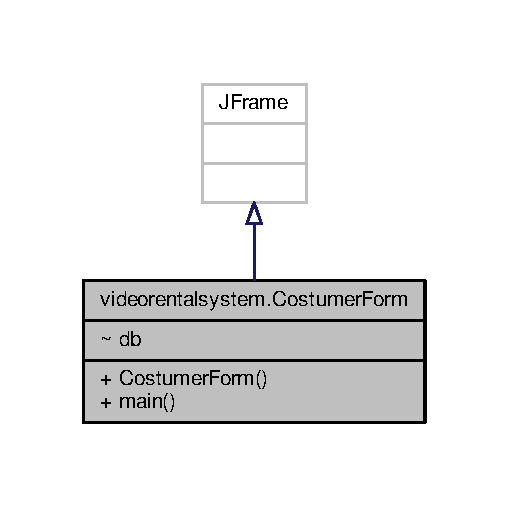
\includegraphics[width=244pt]{classvideorentalsystem_1_1CostumerForm__inherit__graph}
\end{center}
\end{figure}


Collaboration diagram for videorentalsystem.\-Costumer\-Form\-:
\nopagebreak
\begin{figure}[H]
\begin{center}
\leavevmode
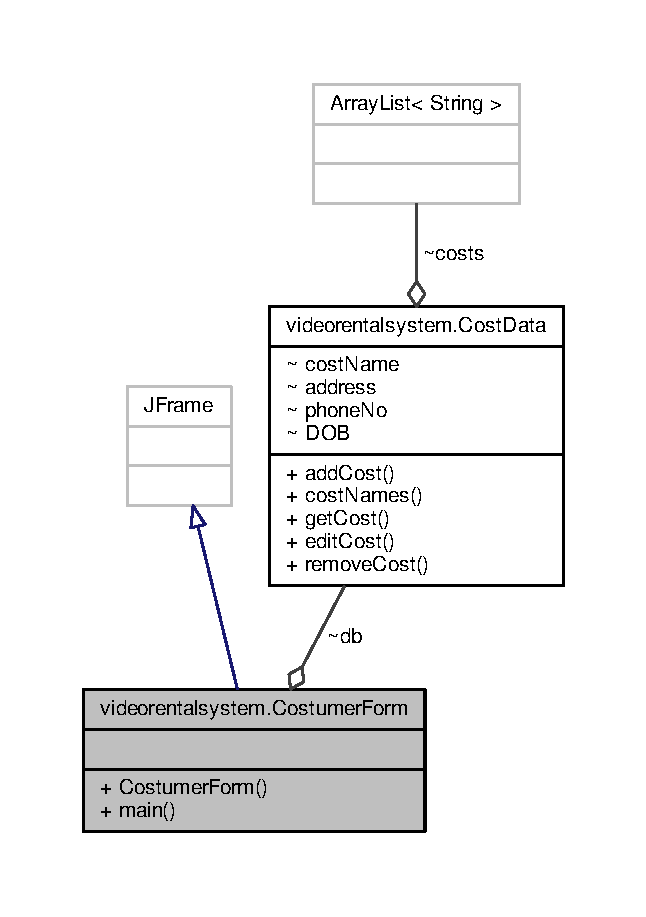
\includegraphics[width=310pt]{classvideorentalsystem_1_1CostumerForm__coll__graph}
\end{center}
\end{figure}
\subsection*{Public Member Functions}
\begin{DoxyCompactItemize}
\item 
\hyperlink{classvideorentalsystem_1_1CostumerForm_aaefba6f9c8bca137b4a806afdd5d2dc3}{Costumer\-Form} ()
\end{DoxyCompactItemize}
\subsection*{Static Public Member Functions}
\begin{DoxyCompactItemize}
\item 
static void \hyperlink{classvideorentalsystem_1_1CostumerForm_a6553f7bdd5d2becfabe09d9d5fc3f8e2}{main} (String args\mbox{[}$\,$\mbox{]})
\end{DoxyCompactItemize}


\subsection{Detailed Description}
\begin{DoxyAuthor}{Author}
user 
\end{DoxyAuthor}


\subsection{Constructor \& Destructor Documentation}
\hypertarget{classvideorentalsystem_1_1CostumerForm_aaefba6f9c8bca137b4a806afdd5d2dc3}{\index{videorentalsystem\-::\-Costumer\-Form@{videorentalsystem\-::\-Costumer\-Form}!Costumer\-Form@{Costumer\-Form}}
\index{Costumer\-Form@{Costumer\-Form}!videorentalsystem::CostumerForm@{videorentalsystem\-::\-Costumer\-Form}}
\subsubsection[{Costumer\-Form}]{\setlength{\rightskip}{0pt plus 5cm}videorentalsystem.\-Costumer\-Form.\-Costumer\-Form (
\begin{DoxyParamCaption}
{}
\end{DoxyParamCaption}
)\hspace{0.3cm}{\ttfamily [inline]}}}\label{classvideorentalsystem_1_1CostumerForm_aaefba6f9c8bca137b4a806afdd5d2dc3}


\subsection{Member Function Documentation}
\hypertarget{classvideorentalsystem_1_1CostumerForm_a6553f7bdd5d2becfabe09d9d5fc3f8e2}{\index{videorentalsystem\-::\-Costumer\-Form@{videorentalsystem\-::\-Costumer\-Form}!main@{main}}
\index{main@{main}!videorentalsystem::CostumerForm@{videorentalsystem\-::\-Costumer\-Form}}
\subsubsection[{main}]{\setlength{\rightskip}{0pt plus 5cm}static void videorentalsystem.\-Costumer\-Form.\-main (
\begin{DoxyParamCaption}
\item[{String}]{args\mbox{[}$\,$\mbox{]}}
\end{DoxyParamCaption}
)\hspace{0.3cm}{\ttfamily [inline]}, {\ttfamily [static]}}}\label{classvideorentalsystem_1_1CostumerForm_a6553f7bdd5d2becfabe09d9d5fc3f8e2}

\begin{DoxyParams}{Parameters}
{\em args} & the command line arguments \\
\hline
\end{DoxyParams}


The documentation for this class was generated from the following file\-:\begin{DoxyCompactItemize}
\item 
\hyperlink{CostumerForm_8java}{Costumer\-Form.\-java}\end{DoxyCompactItemize}

\hypertarget{classvideorentalsystem_1_1Movie}{\section{videorentalsystem.\-Movie Class Reference}
\label{classvideorentalsystem_1_1Movie}\index{videorentalsystem.\-Movie@{videorentalsystem.\-Movie}}
}


Collaboration diagram for videorentalsystem.\-Movie\-:
\nopagebreak
\begin{figure}[H]
\begin{center}
\leavevmode
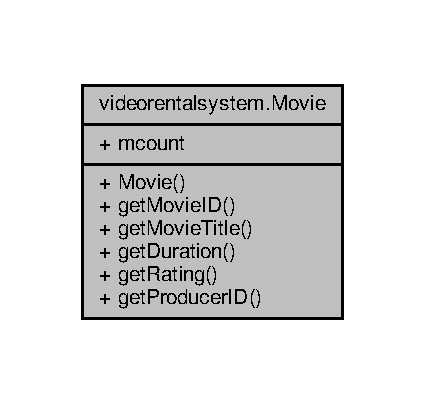
\includegraphics[width=204pt]{classvideorentalsystem_1_1Movie__coll__graph}
\end{center}
\end{figure}
\subsection*{Public Member Functions}
\begin{DoxyCompactItemize}
\item 
\hyperlink{classvideorentalsystem_1_1Movie_aa15a6b662ad8cbdcae50a0e4f4dc2b40}{Movie} (String title, int rating, int duration, int pid)
\item 
int \hyperlink{classvideorentalsystem_1_1Movie_a9174bd5c863d6f53b4cd95c97bb20a6e}{get\-Movie\-I\-D} ()
\item 
String \hyperlink{classvideorentalsystem_1_1Movie_ac32ecf7669f0ab12b51b1e6830b837ca}{get\-Movie\-Title} ()
\item 
int \hyperlink{classvideorentalsystem_1_1Movie_a39a713990661cb3220fc2514b974823d}{get\-Duration} ()
\item 
int \hyperlink{classvideorentalsystem_1_1Movie_a419b38a9fccffc255f3863ad9830df30}{get\-Rating} ()
\item 
int \hyperlink{classvideorentalsystem_1_1Movie_ad96ae53d6d7f646c62e4500625d068ee}{get\-Producer\-I\-D} ()
\end{DoxyCompactItemize}
\subsection*{Static Public Attributes}
\begin{DoxyCompactItemize}
\item 
static int \hyperlink{classvideorentalsystem_1_1Movie_a4b55ef3d24a97727ac317711dd9c7e15}{mcount} =0
\end{DoxyCompactItemize}


\subsection{Detailed Description}
\begin{DoxyAuthor}{Author}
user 
\end{DoxyAuthor}


\subsection{Constructor \& Destructor Documentation}
\hypertarget{classvideorentalsystem_1_1Movie_aa15a6b662ad8cbdcae50a0e4f4dc2b40}{\index{videorentalsystem\-::\-Movie@{videorentalsystem\-::\-Movie}!Movie@{Movie}}
\index{Movie@{Movie}!videorentalsystem::Movie@{videorentalsystem\-::\-Movie}}
\subsubsection[{Movie}]{\setlength{\rightskip}{0pt plus 5cm}videorentalsystem.\-Movie.\-Movie (
\begin{DoxyParamCaption}
\item[{String}]{title, }
\item[{int}]{rating, }
\item[{int}]{duration, }
\item[{int}]{pid}
\end{DoxyParamCaption}
)\hspace{0.3cm}{\ttfamily [inline]}}}\label{classvideorentalsystem_1_1Movie_aa15a6b662ad8cbdcae50a0e4f4dc2b40}


\subsection{Member Function Documentation}
\hypertarget{classvideorentalsystem_1_1Movie_a39a713990661cb3220fc2514b974823d}{\index{videorentalsystem\-::\-Movie@{videorentalsystem\-::\-Movie}!get\-Duration@{get\-Duration}}
\index{get\-Duration@{get\-Duration}!videorentalsystem::Movie@{videorentalsystem\-::\-Movie}}
\subsubsection[{get\-Duration}]{\setlength{\rightskip}{0pt plus 5cm}int videorentalsystem.\-Movie.\-get\-Duration (
\begin{DoxyParamCaption}
{}
\end{DoxyParamCaption}
)\hspace{0.3cm}{\ttfamily [inline]}}}\label{classvideorentalsystem_1_1Movie_a39a713990661cb3220fc2514b974823d}
\hypertarget{classvideorentalsystem_1_1Movie_a9174bd5c863d6f53b4cd95c97bb20a6e}{\index{videorentalsystem\-::\-Movie@{videorentalsystem\-::\-Movie}!get\-Movie\-I\-D@{get\-Movie\-I\-D}}
\index{get\-Movie\-I\-D@{get\-Movie\-I\-D}!videorentalsystem::Movie@{videorentalsystem\-::\-Movie}}
\subsubsection[{get\-Movie\-I\-D}]{\setlength{\rightskip}{0pt plus 5cm}int videorentalsystem.\-Movie.\-get\-Movie\-I\-D (
\begin{DoxyParamCaption}
{}
\end{DoxyParamCaption}
)\hspace{0.3cm}{\ttfamily [inline]}}}\label{classvideorentalsystem_1_1Movie_a9174bd5c863d6f53b4cd95c97bb20a6e}
\hypertarget{classvideorentalsystem_1_1Movie_ac32ecf7669f0ab12b51b1e6830b837ca}{\index{videorentalsystem\-::\-Movie@{videorentalsystem\-::\-Movie}!get\-Movie\-Title@{get\-Movie\-Title}}
\index{get\-Movie\-Title@{get\-Movie\-Title}!videorentalsystem::Movie@{videorentalsystem\-::\-Movie}}
\subsubsection[{get\-Movie\-Title}]{\setlength{\rightskip}{0pt plus 5cm}String videorentalsystem.\-Movie.\-get\-Movie\-Title (
\begin{DoxyParamCaption}
{}
\end{DoxyParamCaption}
)\hspace{0.3cm}{\ttfamily [inline]}}}\label{classvideorentalsystem_1_1Movie_ac32ecf7669f0ab12b51b1e6830b837ca}
\hypertarget{classvideorentalsystem_1_1Movie_ad96ae53d6d7f646c62e4500625d068ee}{\index{videorentalsystem\-::\-Movie@{videorentalsystem\-::\-Movie}!get\-Producer\-I\-D@{get\-Producer\-I\-D}}
\index{get\-Producer\-I\-D@{get\-Producer\-I\-D}!videorentalsystem::Movie@{videorentalsystem\-::\-Movie}}
\subsubsection[{get\-Producer\-I\-D}]{\setlength{\rightskip}{0pt plus 5cm}int videorentalsystem.\-Movie.\-get\-Producer\-I\-D (
\begin{DoxyParamCaption}
{}
\end{DoxyParamCaption}
)\hspace{0.3cm}{\ttfamily [inline]}}}\label{classvideorentalsystem_1_1Movie_ad96ae53d6d7f646c62e4500625d068ee}
\hypertarget{classvideorentalsystem_1_1Movie_a419b38a9fccffc255f3863ad9830df30}{\index{videorentalsystem\-::\-Movie@{videorentalsystem\-::\-Movie}!get\-Rating@{get\-Rating}}
\index{get\-Rating@{get\-Rating}!videorentalsystem::Movie@{videorentalsystem\-::\-Movie}}
\subsubsection[{get\-Rating}]{\setlength{\rightskip}{0pt plus 5cm}int videorentalsystem.\-Movie.\-get\-Rating (
\begin{DoxyParamCaption}
{}
\end{DoxyParamCaption}
)\hspace{0.3cm}{\ttfamily [inline]}}}\label{classvideorentalsystem_1_1Movie_a419b38a9fccffc255f3863ad9830df30}


\subsection{Member Data Documentation}
\hypertarget{classvideorentalsystem_1_1Movie_a4b55ef3d24a97727ac317711dd9c7e15}{\index{videorentalsystem\-::\-Movie@{videorentalsystem\-::\-Movie}!mcount@{mcount}}
\index{mcount@{mcount}!videorentalsystem::Movie@{videorentalsystem\-::\-Movie}}
\subsubsection[{mcount}]{\setlength{\rightskip}{0pt plus 5cm}int videorentalsystem.\-Movie.\-mcount =0\hspace{0.3cm}{\ttfamily [static]}}}\label{classvideorentalsystem_1_1Movie_a4b55ef3d24a97727ac317711dd9c7e15}


The documentation for this class was generated from the following file\-:\begin{DoxyCompactItemize}
\item 
\hyperlink{Movie_8java}{Movie.\-java}\end{DoxyCompactItemize}

\hypertarget{classvideorentalsystem_1_1Producer}{\section{videorentalsystem.\-Producer Class Reference}
\label{classvideorentalsystem_1_1Producer}\index{videorentalsystem.\-Producer@{videorentalsystem.\-Producer}}
}


Collaboration diagram for videorentalsystem.\-Producer\-:
\nopagebreak
\begin{figure}[H]
\begin{center}
\leavevmode
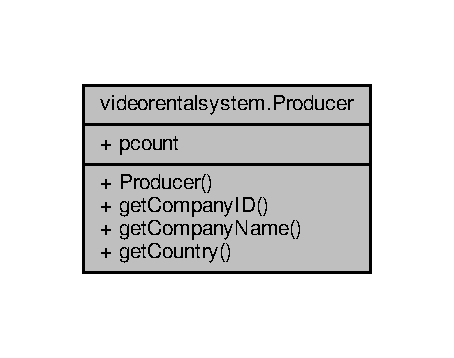
\includegraphics[width=218pt]{classvideorentalsystem_1_1Producer__coll__graph}
\end{center}
\end{figure}
\subsection*{Public Member Functions}
\begin{DoxyCompactItemize}
\item 
\hyperlink{classvideorentalsystem_1_1Producer_a435ae0208121220644dfd1c7434874a6}{Producer} (String cname, String country)
\item 
int \hyperlink{classvideorentalsystem_1_1Producer_a3378b81bdf63bf4be39e5e6ce37fc1c3}{get\-Company\-I\-D} ()
\item 
String \hyperlink{classvideorentalsystem_1_1Producer_a576c7df98eb037be8ba5885c2dfd63fe}{get\-Company\-Name} ()
\item 
String \hyperlink{classvideorentalsystem_1_1Producer_a69158a8988c98fc2517e648cba596a27}{get\-Country} ()
\end{DoxyCompactItemize}
\subsection*{Static Public Attributes}
\begin{DoxyCompactItemize}
\item 
static int \hyperlink{classvideorentalsystem_1_1Producer_af9cea6d53da66d2161104a631a34f093}{pcount} =0
\end{DoxyCompactItemize}


\subsection{Detailed Description}
\begin{DoxyAuthor}{Author}
user 
\end{DoxyAuthor}


\subsection{Constructor \& Destructor Documentation}
\hypertarget{classvideorentalsystem_1_1Producer_a435ae0208121220644dfd1c7434874a6}{\index{videorentalsystem\-::\-Producer@{videorentalsystem\-::\-Producer}!Producer@{Producer}}
\index{Producer@{Producer}!videorentalsystem::Producer@{videorentalsystem\-::\-Producer}}
\subsubsection[{Producer}]{\setlength{\rightskip}{0pt plus 5cm}videorentalsystem.\-Producer.\-Producer (
\begin{DoxyParamCaption}
\item[{String}]{cname, }
\item[{String}]{country}
\end{DoxyParamCaption}
)\hspace{0.3cm}{\ttfamily [inline]}}}\label{classvideorentalsystem_1_1Producer_a435ae0208121220644dfd1c7434874a6}


\subsection{Member Function Documentation}
\hypertarget{classvideorentalsystem_1_1Producer_a3378b81bdf63bf4be39e5e6ce37fc1c3}{\index{videorentalsystem\-::\-Producer@{videorentalsystem\-::\-Producer}!get\-Company\-I\-D@{get\-Company\-I\-D}}
\index{get\-Company\-I\-D@{get\-Company\-I\-D}!videorentalsystem::Producer@{videorentalsystem\-::\-Producer}}
\subsubsection[{get\-Company\-I\-D}]{\setlength{\rightskip}{0pt plus 5cm}int videorentalsystem.\-Producer.\-get\-Company\-I\-D (
\begin{DoxyParamCaption}
{}
\end{DoxyParamCaption}
)\hspace{0.3cm}{\ttfamily [inline]}}}\label{classvideorentalsystem_1_1Producer_a3378b81bdf63bf4be39e5e6ce37fc1c3}
\hypertarget{classvideorentalsystem_1_1Producer_a576c7df98eb037be8ba5885c2dfd63fe}{\index{videorentalsystem\-::\-Producer@{videorentalsystem\-::\-Producer}!get\-Company\-Name@{get\-Company\-Name}}
\index{get\-Company\-Name@{get\-Company\-Name}!videorentalsystem::Producer@{videorentalsystem\-::\-Producer}}
\subsubsection[{get\-Company\-Name}]{\setlength{\rightskip}{0pt plus 5cm}String videorentalsystem.\-Producer.\-get\-Company\-Name (
\begin{DoxyParamCaption}
{}
\end{DoxyParamCaption}
)\hspace{0.3cm}{\ttfamily [inline]}}}\label{classvideorentalsystem_1_1Producer_a576c7df98eb037be8ba5885c2dfd63fe}
\hypertarget{classvideorentalsystem_1_1Producer_a69158a8988c98fc2517e648cba596a27}{\index{videorentalsystem\-::\-Producer@{videorentalsystem\-::\-Producer}!get\-Country@{get\-Country}}
\index{get\-Country@{get\-Country}!videorentalsystem::Producer@{videorentalsystem\-::\-Producer}}
\subsubsection[{get\-Country}]{\setlength{\rightskip}{0pt plus 5cm}String videorentalsystem.\-Producer.\-get\-Country (
\begin{DoxyParamCaption}
{}
\end{DoxyParamCaption}
)\hspace{0.3cm}{\ttfamily [inline]}}}\label{classvideorentalsystem_1_1Producer_a69158a8988c98fc2517e648cba596a27}


\subsection{Member Data Documentation}
\hypertarget{classvideorentalsystem_1_1Producer_af9cea6d53da66d2161104a631a34f093}{\index{videorentalsystem\-::\-Producer@{videorentalsystem\-::\-Producer}!pcount@{pcount}}
\index{pcount@{pcount}!videorentalsystem::Producer@{videorentalsystem\-::\-Producer}}
\subsubsection[{pcount}]{\setlength{\rightskip}{0pt plus 5cm}int videorentalsystem.\-Producer.\-pcount =0\hspace{0.3cm}{\ttfamily [static]}}}\label{classvideorentalsystem_1_1Producer_af9cea6d53da66d2161104a631a34f093}


The documentation for this class was generated from the following file\-:\begin{DoxyCompactItemize}
\item 
\hyperlink{Producer_8java}{Producer.\-java}\end{DoxyCompactItemize}

\hypertarget{classvideorentalsystem_1_1Rental}{\section{videorentalsystem.\-Rental Class Reference}
\label{classvideorentalsystem_1_1Rental}\index{videorentalsystem.\-Rental@{videorentalsystem.\-Rental}}
}


Collaboration diagram for videorentalsystem.\-Rental\-:
\nopagebreak
\begin{figure}[H]
\begin{center}
\leavevmode
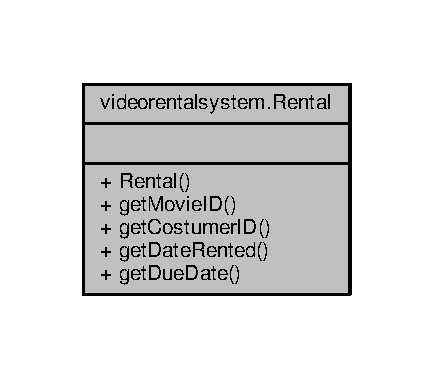
\includegraphics[width=208pt]{classvideorentalsystem_1_1Rental__coll__graph}
\end{center}
\end{figure}
\subsection*{Public Member Functions}
\begin{DoxyCompactItemize}
\item 
\hyperlink{classvideorentalsystem_1_1Rental_af7a54279ae3d0f23c4bf153697328dc1}{Rental} (int mid, int cid, String dr, String dd)
\item 
int \hyperlink{classvideorentalsystem_1_1Rental_a5193f532b28c06ad36988e0704e8a57d}{get\-Movie\-I\-D} ()
\item 
int \hyperlink{classvideorentalsystem_1_1Rental_ac14f266fe0f4b36785b9cf0e9c47b4d8}{get\-Costumer\-I\-D} ()
\item 
String \hyperlink{classvideorentalsystem_1_1Rental_a44ad71775fe6496742da543e3129aebb}{get\-Date\-Rented} ()
\item 
String \hyperlink{classvideorentalsystem_1_1Rental_a3ed76e0212907fa402a58f9b983db82e}{get\-Due\-Date} ()
\end{DoxyCompactItemize}


\subsection{Detailed Description}
\begin{DoxyAuthor}{Author}
user 
\end{DoxyAuthor}


\subsection{Constructor \& Destructor Documentation}
\hypertarget{classvideorentalsystem_1_1Rental_af7a54279ae3d0f23c4bf153697328dc1}{\index{videorentalsystem\-::\-Rental@{videorentalsystem\-::\-Rental}!Rental@{Rental}}
\index{Rental@{Rental}!videorentalsystem::Rental@{videorentalsystem\-::\-Rental}}
\subsubsection[{Rental}]{\setlength{\rightskip}{0pt plus 5cm}videorentalsystem.\-Rental.\-Rental (
\begin{DoxyParamCaption}
\item[{int}]{mid, }
\item[{int}]{cid, }
\item[{String}]{dr, }
\item[{String}]{dd}
\end{DoxyParamCaption}
)\hspace{0.3cm}{\ttfamily [inline]}}}\label{classvideorentalsystem_1_1Rental_af7a54279ae3d0f23c4bf153697328dc1}


\subsection{Member Function Documentation}
\hypertarget{classvideorentalsystem_1_1Rental_ac14f266fe0f4b36785b9cf0e9c47b4d8}{\index{videorentalsystem\-::\-Rental@{videorentalsystem\-::\-Rental}!get\-Costumer\-I\-D@{get\-Costumer\-I\-D}}
\index{get\-Costumer\-I\-D@{get\-Costumer\-I\-D}!videorentalsystem::Rental@{videorentalsystem\-::\-Rental}}
\subsubsection[{get\-Costumer\-I\-D}]{\setlength{\rightskip}{0pt plus 5cm}int videorentalsystem.\-Rental.\-get\-Costumer\-I\-D (
\begin{DoxyParamCaption}
{}
\end{DoxyParamCaption}
)\hspace{0.3cm}{\ttfamily [inline]}}}\label{classvideorentalsystem_1_1Rental_ac14f266fe0f4b36785b9cf0e9c47b4d8}
\hypertarget{classvideorentalsystem_1_1Rental_a44ad71775fe6496742da543e3129aebb}{\index{videorentalsystem\-::\-Rental@{videorentalsystem\-::\-Rental}!get\-Date\-Rented@{get\-Date\-Rented}}
\index{get\-Date\-Rented@{get\-Date\-Rented}!videorentalsystem::Rental@{videorentalsystem\-::\-Rental}}
\subsubsection[{get\-Date\-Rented}]{\setlength{\rightskip}{0pt plus 5cm}String videorentalsystem.\-Rental.\-get\-Date\-Rented (
\begin{DoxyParamCaption}
{}
\end{DoxyParamCaption}
)\hspace{0.3cm}{\ttfamily [inline]}}}\label{classvideorentalsystem_1_1Rental_a44ad71775fe6496742da543e3129aebb}
\hypertarget{classvideorentalsystem_1_1Rental_a3ed76e0212907fa402a58f9b983db82e}{\index{videorentalsystem\-::\-Rental@{videorentalsystem\-::\-Rental}!get\-Due\-Date@{get\-Due\-Date}}
\index{get\-Due\-Date@{get\-Due\-Date}!videorentalsystem::Rental@{videorentalsystem\-::\-Rental}}
\subsubsection[{get\-Due\-Date}]{\setlength{\rightskip}{0pt plus 5cm}String videorentalsystem.\-Rental.\-get\-Due\-Date (
\begin{DoxyParamCaption}
{}
\end{DoxyParamCaption}
)\hspace{0.3cm}{\ttfamily [inline]}}}\label{classvideorentalsystem_1_1Rental_a3ed76e0212907fa402a58f9b983db82e}
\hypertarget{classvideorentalsystem_1_1Rental_a5193f532b28c06ad36988e0704e8a57d}{\index{videorentalsystem\-::\-Rental@{videorentalsystem\-::\-Rental}!get\-Movie\-I\-D@{get\-Movie\-I\-D}}
\index{get\-Movie\-I\-D@{get\-Movie\-I\-D}!videorentalsystem::Rental@{videorentalsystem\-::\-Rental}}
\subsubsection[{get\-Movie\-I\-D}]{\setlength{\rightskip}{0pt plus 5cm}int videorentalsystem.\-Rental.\-get\-Movie\-I\-D (
\begin{DoxyParamCaption}
{}
\end{DoxyParamCaption}
)\hspace{0.3cm}{\ttfamily [inline]}}}\label{classvideorentalsystem_1_1Rental_a5193f532b28c06ad36988e0704e8a57d}


The documentation for this class was generated from the following file\-:\begin{DoxyCompactItemize}
\item 
\hyperlink{Rental_8java}{Rental.\-java}\end{DoxyCompactItemize}

\hypertarget{classvideorentalsystem_1_1RentVideo}{\section{videorentalsystem.\-Rent\-Video Class Reference}
\label{classvideorentalsystem_1_1RentVideo}\index{videorentalsystem.\-Rent\-Video@{videorentalsystem.\-Rent\-Video}}
}


Inheritance diagram for videorentalsystem.\-Rent\-Video\-:
\nopagebreak
\begin{figure}[H]
\begin{center}
\leavevmode
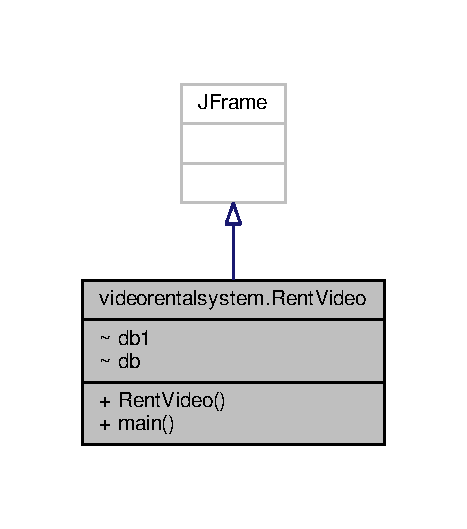
\includegraphics[width=224pt]{classvideorentalsystem_1_1RentVideo__inherit__graph}
\end{center}
\end{figure}


Collaboration diagram for videorentalsystem.\-Rent\-Video\-:
\nopagebreak
\begin{figure}[H]
\begin{center}
\leavevmode
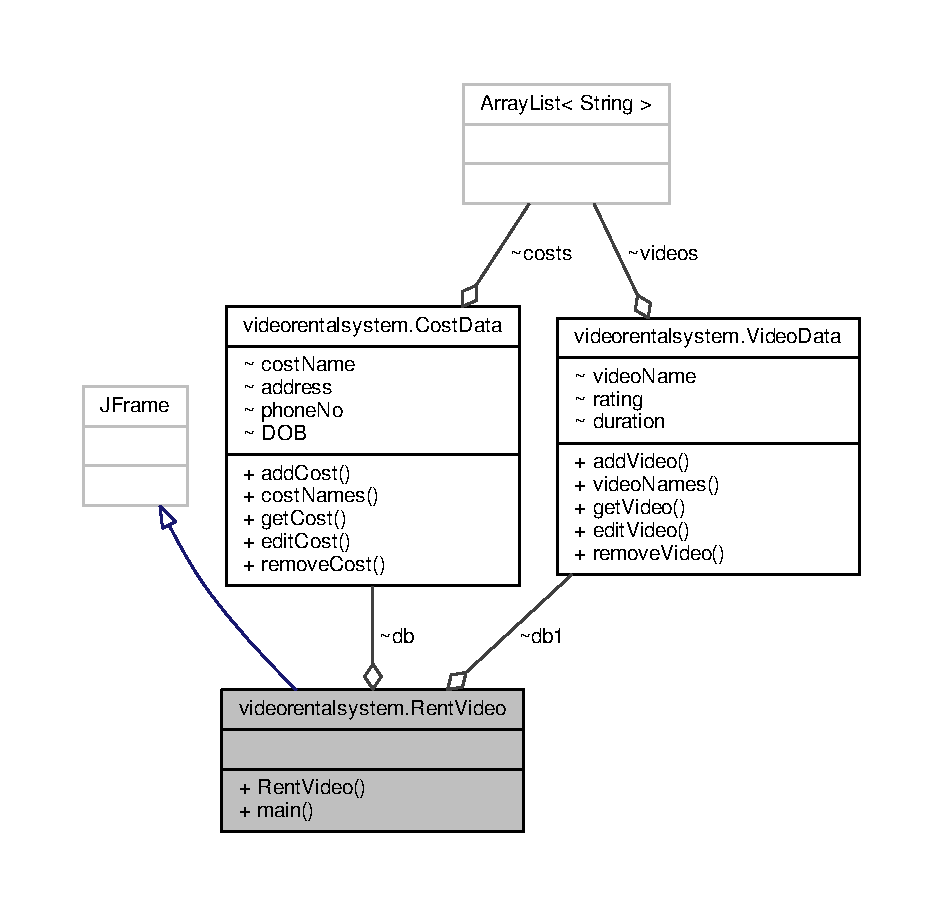
\includegraphics[width=350pt]{classvideorentalsystem_1_1RentVideo__coll__graph}
\end{center}
\end{figure}
\subsection*{Public Member Functions}
\begin{DoxyCompactItemize}
\item 
\hyperlink{classvideorentalsystem_1_1RentVideo_a1b7721eddd9ad7ec2e1c8ce8fb80d181}{Rent\-Video} ()
\end{DoxyCompactItemize}
\subsection*{Static Public Member Functions}
\begin{DoxyCompactItemize}
\item 
static void \hyperlink{classvideorentalsystem_1_1RentVideo_a8b38b8b61939d68f5f5802b91e40743c}{main} (String args\mbox{[}$\,$\mbox{]})
\end{DoxyCompactItemize}


\subsection{Detailed Description}
\begin{DoxyAuthor}{Author}
user 
\end{DoxyAuthor}


\subsection{Constructor \& Destructor Documentation}
\hypertarget{classvideorentalsystem_1_1RentVideo_a1b7721eddd9ad7ec2e1c8ce8fb80d181}{\index{videorentalsystem\-::\-Rent\-Video@{videorentalsystem\-::\-Rent\-Video}!Rent\-Video@{Rent\-Video}}
\index{Rent\-Video@{Rent\-Video}!videorentalsystem::RentVideo@{videorentalsystem\-::\-Rent\-Video}}
\subsubsection[{Rent\-Video}]{\setlength{\rightskip}{0pt plus 5cm}videorentalsystem.\-Rent\-Video.\-Rent\-Video (
\begin{DoxyParamCaption}
{}
\end{DoxyParamCaption}
)\hspace{0.3cm}{\ttfamily [inline]}}}\label{classvideorentalsystem_1_1RentVideo_a1b7721eddd9ad7ec2e1c8ce8fb80d181}


\subsection{Member Function Documentation}
\hypertarget{classvideorentalsystem_1_1RentVideo_a8b38b8b61939d68f5f5802b91e40743c}{\index{videorentalsystem\-::\-Rent\-Video@{videorentalsystem\-::\-Rent\-Video}!main@{main}}
\index{main@{main}!videorentalsystem::RentVideo@{videorentalsystem\-::\-Rent\-Video}}
\subsubsection[{main}]{\setlength{\rightskip}{0pt plus 5cm}static void videorentalsystem.\-Rent\-Video.\-main (
\begin{DoxyParamCaption}
\item[{String}]{args\mbox{[}$\,$\mbox{]}}
\end{DoxyParamCaption}
)\hspace{0.3cm}{\ttfamily [inline]}, {\ttfamily [static]}}}\label{classvideorentalsystem_1_1RentVideo_a8b38b8b61939d68f5f5802b91e40743c}

\begin{DoxyParams}{Parameters}
{\em args} & the command line arguments \\
\hline
\end{DoxyParams}


The documentation for this class was generated from the following file\-:\begin{DoxyCompactItemize}
\item 
\hyperlink{RentVideo_8java}{Rent\-Video.\-java}\end{DoxyCompactItemize}

\hypertarget{classvideorentalsystem_1_1VideoData}{\section{videorentalsystem.\-Video\-Data Class Reference}
\label{classvideorentalsystem_1_1VideoData}\index{videorentalsystem.\-Video\-Data@{videorentalsystem.\-Video\-Data}}
}


Collaboration diagram for videorentalsystem.\-Video\-Data\-:
\nopagebreak
\begin{figure}[H]
\begin{center}
\leavevmode
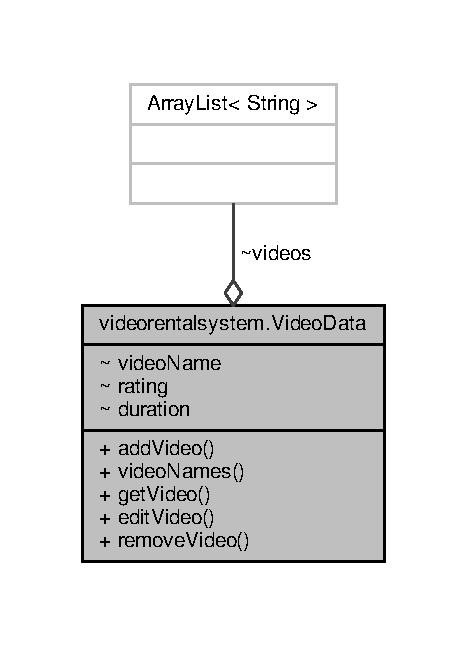
\includegraphics[width=224pt]{classvideorentalsystem_1_1VideoData__coll__graph}
\end{center}
\end{figure}
\subsection*{Public Member Functions}
\begin{DoxyCompactItemize}
\item 
void \hyperlink{classvideorentalsystem_1_1VideoData_a2eafb84494d23316076baf7a02c9ef6b}{add\-Video} (String video\-Name, String rating, String duration)
\item 
Array\-List$<$ String $>$ \hyperlink{classvideorentalsystem_1_1VideoData_ae922fd11560964f9921fa83b4153deef}{video\-Names} ()
\item 
void \hyperlink{classvideorentalsystem_1_1VideoData_abc5353826530e5a91cf9a83a9bdbef57}{get\-Video} (String video\-Name)
\item 
void \hyperlink{classvideorentalsystem_1_1VideoData_a6eb6534b7bb975b801172d7e45b5abbe}{edit\-Video} (String oldvideo\-Name, String newvideo\-Name, String duration, String rating)
\item 
void \hyperlink{classvideorentalsystem_1_1VideoData_a77480f24c0d089793233daf4378dd75f}{remove\-Video} (String video\-Name)
\end{DoxyCompactItemize}


\subsection{Detailed Description}
\begin{DoxyAuthor}{Author}
abhinav 
\end{DoxyAuthor}


\subsection{Member Function Documentation}
\hypertarget{classvideorentalsystem_1_1VideoData_a2eafb84494d23316076baf7a02c9ef6b}{\index{videorentalsystem\-::\-Video\-Data@{videorentalsystem\-::\-Video\-Data}!add\-Video@{add\-Video}}
\index{add\-Video@{add\-Video}!videorentalsystem::VideoData@{videorentalsystem\-::\-Video\-Data}}
\subsubsection[{add\-Video}]{\setlength{\rightskip}{0pt plus 5cm}void videorentalsystem.\-Video\-Data.\-add\-Video (
\begin{DoxyParamCaption}
\item[{String}]{video\-Name, }
\item[{String}]{rating, }
\item[{String}]{duration}
\end{DoxyParamCaption}
)\hspace{0.3cm}{\ttfamily [inline]}}}\label{classvideorentalsystem_1_1VideoData_a2eafb84494d23316076baf7a02c9ef6b}
\hypertarget{classvideorentalsystem_1_1VideoData_a6eb6534b7bb975b801172d7e45b5abbe}{\index{videorentalsystem\-::\-Video\-Data@{videorentalsystem\-::\-Video\-Data}!edit\-Video@{edit\-Video}}
\index{edit\-Video@{edit\-Video}!videorentalsystem::VideoData@{videorentalsystem\-::\-Video\-Data}}
\subsubsection[{edit\-Video}]{\setlength{\rightskip}{0pt plus 5cm}void videorentalsystem.\-Video\-Data.\-edit\-Video (
\begin{DoxyParamCaption}
\item[{String}]{oldvideo\-Name, }
\item[{String}]{newvideo\-Name, }
\item[{String}]{duration, }
\item[{String}]{rating}
\end{DoxyParamCaption}
)\hspace{0.3cm}{\ttfamily [inline]}}}\label{classvideorentalsystem_1_1VideoData_a6eb6534b7bb975b801172d7e45b5abbe}
\hypertarget{classvideorentalsystem_1_1VideoData_abc5353826530e5a91cf9a83a9bdbef57}{\index{videorentalsystem\-::\-Video\-Data@{videorentalsystem\-::\-Video\-Data}!get\-Video@{get\-Video}}
\index{get\-Video@{get\-Video}!videorentalsystem::VideoData@{videorentalsystem\-::\-Video\-Data}}
\subsubsection[{get\-Video}]{\setlength{\rightskip}{0pt plus 5cm}void videorentalsystem.\-Video\-Data.\-get\-Video (
\begin{DoxyParamCaption}
\item[{String}]{video\-Name}
\end{DoxyParamCaption}
)\hspace{0.3cm}{\ttfamily [inline]}}}\label{classvideorentalsystem_1_1VideoData_abc5353826530e5a91cf9a83a9bdbef57}
\hypertarget{classvideorentalsystem_1_1VideoData_a77480f24c0d089793233daf4378dd75f}{\index{videorentalsystem\-::\-Video\-Data@{videorentalsystem\-::\-Video\-Data}!remove\-Video@{remove\-Video}}
\index{remove\-Video@{remove\-Video}!videorentalsystem::VideoData@{videorentalsystem\-::\-Video\-Data}}
\subsubsection[{remove\-Video}]{\setlength{\rightskip}{0pt plus 5cm}void videorentalsystem.\-Video\-Data.\-remove\-Video (
\begin{DoxyParamCaption}
\item[{String}]{video\-Name}
\end{DoxyParamCaption}
)\hspace{0.3cm}{\ttfamily [inline]}}}\label{classvideorentalsystem_1_1VideoData_a77480f24c0d089793233daf4378dd75f}
\hypertarget{classvideorentalsystem_1_1VideoData_ae922fd11560964f9921fa83b4153deef}{\index{videorentalsystem\-::\-Video\-Data@{videorentalsystem\-::\-Video\-Data}!video\-Names@{video\-Names}}
\index{video\-Names@{video\-Names}!videorentalsystem::VideoData@{videorentalsystem\-::\-Video\-Data}}
\subsubsection[{video\-Names}]{\setlength{\rightskip}{0pt plus 5cm}Array\-List$<$String$>$ videorentalsystem.\-Video\-Data.\-video\-Names (
\begin{DoxyParamCaption}
{}
\end{DoxyParamCaption}
)\hspace{0.3cm}{\ttfamily [inline]}}}\label{classvideorentalsystem_1_1VideoData_ae922fd11560964f9921fa83b4153deef}


The documentation for this class was generated from the following file\-:\begin{DoxyCompactItemize}
\item 
\hyperlink{VideoData_8java}{Video\-Data.\-java}\end{DoxyCompactItemize}

\hypertarget{classvideorentalsystem_1_1VideoForm}{\section{videorentalsystem.\-Video\-Form Class Reference}
\label{classvideorentalsystem_1_1VideoForm}\index{videorentalsystem.\-Video\-Form@{videorentalsystem.\-Video\-Form}}
}


Inheritance diagram for videorentalsystem.\-Video\-Form\-:
\nopagebreak
\begin{figure}[H]
\begin{center}
\leavevmode
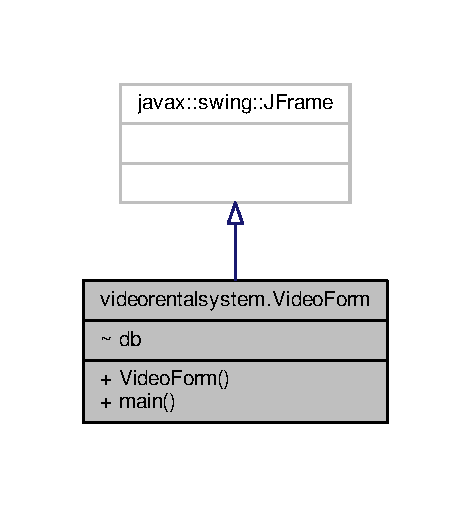
\includegraphics[width=226pt]{classvideorentalsystem_1_1VideoForm__inherit__graph}
\end{center}
\end{figure}


Collaboration diagram for videorentalsystem.\-Video\-Form\-:
\nopagebreak
\begin{figure}[H]
\begin{center}
\leavevmode
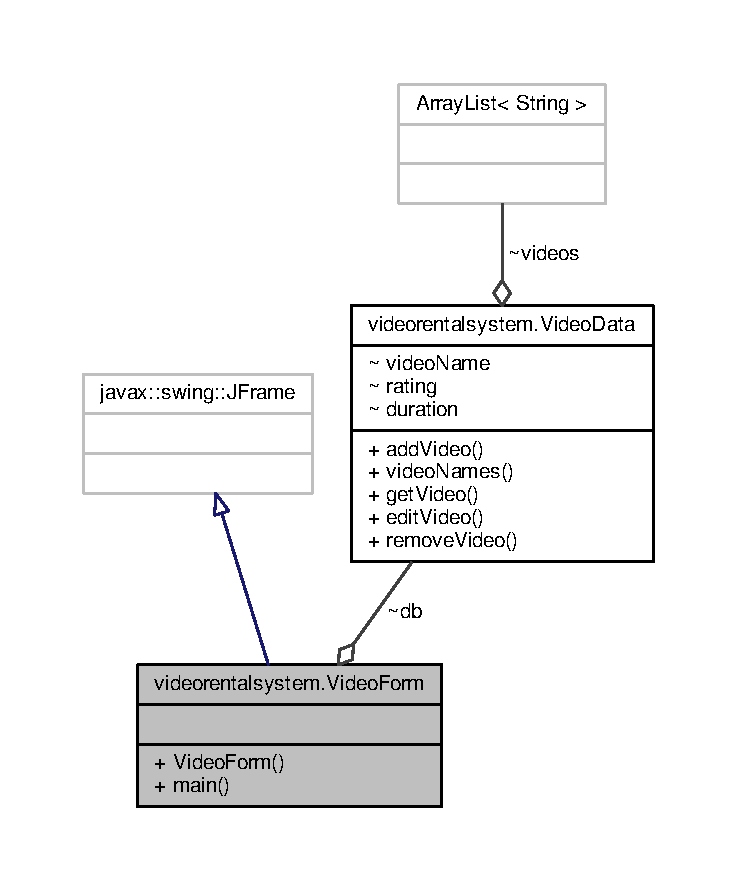
\includegraphics[width=350pt]{classvideorentalsystem_1_1VideoForm__coll__graph}
\end{center}
\end{figure}
\subsection*{Public Member Functions}
\begin{DoxyCompactItemize}
\item 
\hyperlink{classvideorentalsystem_1_1VideoForm_aab99df615d3ee1ede6610865c3de4d24}{Video\-Form} ()
\end{DoxyCompactItemize}
\subsection*{Static Public Member Functions}
\begin{DoxyCompactItemize}
\item 
static void \hyperlink{classvideorentalsystem_1_1VideoForm_a9809e72aae5f98338e62e4d1751c331c}{main} (String args\mbox{[}$\,$\mbox{]})
\end{DoxyCompactItemize}


\subsection{Detailed Description}
\begin{DoxyAuthor}{Author}
user 
\end{DoxyAuthor}


\subsection{Constructor \& Destructor Documentation}
\hypertarget{classvideorentalsystem_1_1VideoForm_aab99df615d3ee1ede6610865c3de4d24}{\index{videorentalsystem\-::\-Video\-Form@{videorentalsystem\-::\-Video\-Form}!Video\-Form@{Video\-Form}}
\index{Video\-Form@{Video\-Form}!videorentalsystem::VideoForm@{videorentalsystem\-::\-Video\-Form}}
\subsubsection[{Video\-Form}]{\setlength{\rightskip}{0pt plus 5cm}videorentalsystem.\-Video\-Form.\-Video\-Form (
\begin{DoxyParamCaption}
{}
\end{DoxyParamCaption}
)\hspace{0.3cm}{\ttfamily [inline]}}}\label{classvideorentalsystem_1_1VideoForm_aab99df615d3ee1ede6610865c3de4d24}


\subsection{Member Function Documentation}
\hypertarget{classvideorentalsystem_1_1VideoForm_a9809e72aae5f98338e62e4d1751c331c}{\index{videorentalsystem\-::\-Video\-Form@{videorentalsystem\-::\-Video\-Form}!main@{main}}
\index{main@{main}!videorentalsystem::VideoForm@{videorentalsystem\-::\-Video\-Form}}
\subsubsection[{main}]{\setlength{\rightskip}{0pt plus 5cm}static void videorentalsystem.\-Video\-Form.\-main (
\begin{DoxyParamCaption}
\item[{String}]{args\mbox{[}$\,$\mbox{]}}
\end{DoxyParamCaption}
)\hspace{0.3cm}{\ttfamily [inline]}, {\ttfamily [static]}}}\label{classvideorentalsystem_1_1VideoForm_a9809e72aae5f98338e62e4d1751c331c}

\begin{DoxyParams}{Parameters}
{\em args} & the command line arguments \\
\hline
\end{DoxyParams}


The documentation for this class was generated from the following file\-:\begin{DoxyCompactItemize}
\item 
\hyperlink{VideoForm_8java}{Video\-Form.\-java}\end{DoxyCompactItemize}

\hypertarget{classvideorentalsystem_1_1VideoRentalSystem}{\section{videorentalsystem.\-Video\-Rental\-System Class Reference}
\label{classvideorentalsystem_1_1VideoRentalSystem}\index{videorentalsystem.\-Video\-Rental\-System@{videorentalsystem.\-Video\-Rental\-System}}
}


Collaboration diagram for videorentalsystem.\-Video\-Rental\-System\-:
\nopagebreak
\begin{figure}[H]
\begin{center}
\leavevmode
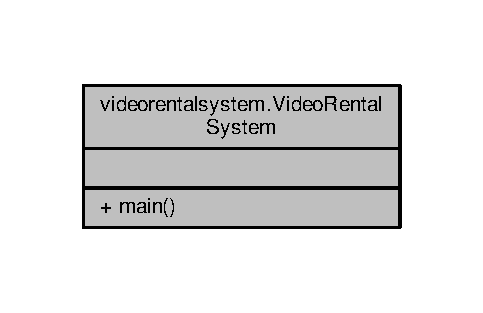
\includegraphics[width=232pt]{classvideorentalsystem_1_1VideoRentalSystem__coll__graph}
\end{center}
\end{figure}
\subsection*{Static Public Member Functions}
\begin{DoxyCompactItemize}
\item 
static void \hyperlink{classvideorentalsystem_1_1VideoRentalSystem_ac971f52492b5adb76d2c81a6a29220cc}{main} (String\mbox{[}$\,$\mbox{]} args)
\end{DoxyCompactItemize}


\subsection{Detailed Description}
\begin{DoxyAuthor}{Author}
abhinav 
\end{DoxyAuthor}


\subsection{Member Function Documentation}
\hypertarget{classvideorentalsystem_1_1VideoRentalSystem_ac971f52492b5adb76d2c81a6a29220cc}{\index{videorentalsystem\-::\-Video\-Rental\-System@{videorentalsystem\-::\-Video\-Rental\-System}!main@{main}}
\index{main@{main}!videorentalsystem::VideoRentalSystem@{videorentalsystem\-::\-Video\-Rental\-System}}
\subsubsection[{main}]{\setlength{\rightskip}{0pt plus 5cm}static void videorentalsystem.\-Video\-Rental\-System.\-main (
\begin{DoxyParamCaption}
\item[{String\mbox{[}$\,$\mbox{]}}]{args}
\end{DoxyParamCaption}
)\hspace{0.3cm}{\ttfamily [inline]}, {\ttfamily [static]}}}\label{classvideorentalsystem_1_1VideoRentalSystem_ac971f52492b5adb76d2c81a6a29220cc}


The documentation for this class was generated from the following file\-:\begin{DoxyCompactItemize}
\item 
\hyperlink{VideoRentalSystem_8java}{Video\-Rental\-System.\-java}\end{DoxyCompactItemize}

\hypertarget{classvideorentalsystem_1_1Welcome}{\section{videorentalsystem.\-Welcome Class Reference}
\label{classvideorentalsystem_1_1Welcome}\index{videorentalsystem.\-Welcome@{videorentalsystem.\-Welcome}}
}


Inheritance diagram for videorentalsystem.\-Welcome\-:
\nopagebreak
\begin{figure}[H]
\begin{center}
\leavevmode
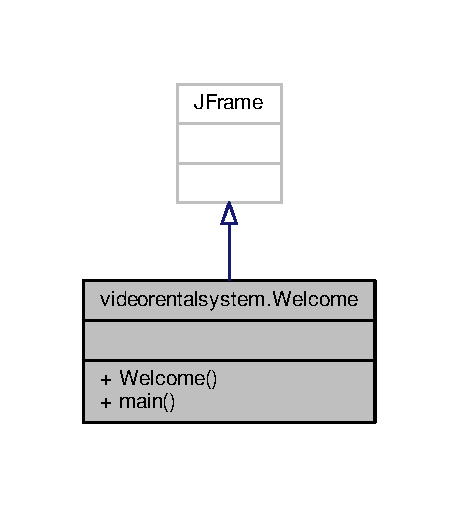
\includegraphics[width=220pt]{classvideorentalsystem_1_1Welcome__inherit__graph}
\end{center}
\end{figure}


Collaboration diagram for videorentalsystem.\-Welcome\-:
\nopagebreak
\begin{figure}[H]
\begin{center}
\leavevmode
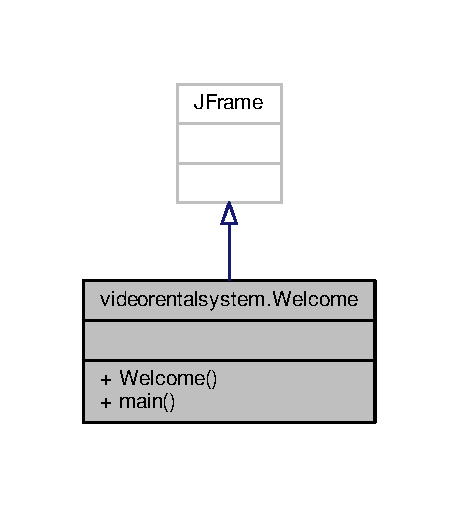
\includegraphics[width=220pt]{classvideorentalsystem_1_1Welcome__coll__graph}
\end{center}
\end{figure}
\subsection*{Public Member Functions}
\begin{DoxyCompactItemize}
\item 
\hyperlink{classvideorentalsystem_1_1Welcome_ad88f2e69e90df3af70729162f98639bf}{Welcome} ()
\end{DoxyCompactItemize}
\subsection*{Static Public Member Functions}
\begin{DoxyCompactItemize}
\item 
static void \hyperlink{classvideorentalsystem_1_1Welcome_a0eac89994aa30e08d5c9eb0199802213}{main} (String args\mbox{[}$\,$\mbox{]})
\end{DoxyCompactItemize}


\subsection{Detailed Description}
\begin{DoxyAuthor}{Author}
user 
\end{DoxyAuthor}


\subsection{Constructor \& Destructor Documentation}
\hypertarget{classvideorentalsystem_1_1Welcome_ad88f2e69e90df3af70729162f98639bf}{\index{videorentalsystem\-::\-Welcome@{videorentalsystem\-::\-Welcome}!Welcome@{Welcome}}
\index{Welcome@{Welcome}!videorentalsystem::Welcome@{videorentalsystem\-::\-Welcome}}
\subsubsection[{Welcome}]{\setlength{\rightskip}{0pt plus 5cm}videorentalsystem.\-Welcome.\-Welcome (
\begin{DoxyParamCaption}
{}
\end{DoxyParamCaption}
)\hspace{0.3cm}{\ttfamily [inline]}}}\label{classvideorentalsystem_1_1Welcome_ad88f2e69e90df3af70729162f98639bf}
Creates new form \hyperlink{classvideorentalsystem_1_1Welcome}{Welcome} 

\subsection{Member Function Documentation}
\hypertarget{classvideorentalsystem_1_1Welcome_a0eac89994aa30e08d5c9eb0199802213}{\index{videorentalsystem\-::\-Welcome@{videorentalsystem\-::\-Welcome}!main@{main}}
\index{main@{main}!videorentalsystem::Welcome@{videorentalsystem\-::\-Welcome}}
\subsubsection[{main}]{\setlength{\rightskip}{0pt plus 5cm}static void videorentalsystem.\-Welcome.\-main (
\begin{DoxyParamCaption}
\item[{String}]{args\mbox{[}$\,$\mbox{]}}
\end{DoxyParamCaption}
)\hspace{0.3cm}{\ttfamily [inline]}, {\ttfamily [static]}}}\label{classvideorentalsystem_1_1Welcome_a0eac89994aa30e08d5c9eb0199802213}

\begin{DoxyParams}{Parameters}
{\em args} & the command line arguments \\
\hline
\end{DoxyParams}


The documentation for this class was generated from the following file\-:\begin{DoxyCompactItemize}
\item 
\hyperlink{Welcome_8java}{Welcome.\-java}\end{DoxyCompactItemize}

\chapter{File Documentation}
\hypertarget{CostData_8java}{\section{Cost\-Data.\-java File Reference}
\label{CostData_8java}\index{Cost\-Data.\-java@{Cost\-Data.\-java}}
}
\subsection*{Classes}
\begin{DoxyCompactItemize}
\item 
class \hyperlink{classvideorentalsystem_1_1CostData}{videorentalsystem.\-Cost\-Data}
\end{DoxyCompactItemize}
\subsection*{Packages}
\begin{DoxyCompactItemize}
\item 
package \hyperlink{namespacevideorentalsystem}{videorentalsystem}
\end{DoxyCompactItemize}

\hypertarget{Costumer_8java}{\section{Costumer.\-java File Reference}
\label{Costumer_8java}\index{Costumer.\-java@{Costumer.\-java}}
}
\subsection*{Classes}
\begin{DoxyCompactItemize}
\item 
class \hyperlink{classvideorentalsystem_1_1Costumer}{videorentalsystem.\-Costumer}
\end{DoxyCompactItemize}
\subsection*{Packages}
\begin{DoxyCompactItemize}
\item 
package \hyperlink{namespacevideorentalsystem}{videorentalsystem}
\end{DoxyCompactItemize}

\hypertarget{CostumerForm_8java}{\section{Costumer\-Form.\-java File Reference}
\label{CostumerForm_8java}\index{Costumer\-Form.\-java@{Costumer\-Form.\-java}}
}
\subsection*{Classes}
\begin{DoxyCompactItemize}
\item 
class \hyperlink{classvideorentalsystem_1_1CostumerForm}{videorentalsystem.\-Costumer\-Form}
\end{DoxyCompactItemize}
\subsection*{Packages}
\begin{DoxyCompactItemize}
\item 
package \hyperlink{namespacevideorentalsystem}{videorentalsystem}
\end{DoxyCompactItemize}

\hypertarget{Movie_8java}{\section{Movie.\-java File Reference}
\label{Movie_8java}\index{Movie.\-java@{Movie.\-java}}
}
\subsection*{Classes}
\begin{DoxyCompactItemize}
\item 
class \hyperlink{classvideorentalsystem_1_1Movie}{videorentalsystem.\-Movie}
\end{DoxyCompactItemize}
\subsection*{Packages}
\begin{DoxyCompactItemize}
\item 
package \hyperlink{namespacevideorentalsystem}{videorentalsystem}
\end{DoxyCompactItemize}

\hypertarget{Producer_8java}{\section{Producer.\-java File Reference}
\label{Producer_8java}\index{Producer.\-java@{Producer.\-java}}
}
\subsection*{Classes}
\begin{DoxyCompactItemize}
\item 
class \hyperlink{classvideorentalsystem_1_1Producer}{videorentalsystem.\-Producer}
\end{DoxyCompactItemize}
\subsection*{Packages}
\begin{DoxyCompactItemize}
\item 
package \hyperlink{namespacevideorentalsystem}{videorentalsystem}
\end{DoxyCompactItemize}

\hypertarget{Rental_8java}{\section{Rental.\-java File Reference}
\label{Rental_8java}\index{Rental.\-java@{Rental.\-java}}
}
\subsection*{Classes}
\begin{DoxyCompactItemize}
\item 
class \hyperlink{classvideorentalsystem_1_1Rental}{videorentalsystem.\-Rental}
\end{DoxyCompactItemize}
\subsection*{Packages}
\begin{DoxyCompactItemize}
\item 
package \hyperlink{namespacevideorentalsystem}{videorentalsystem}
\end{DoxyCompactItemize}

\hypertarget{RentVideo_8java}{\section{Rent\-Video.\-java File Reference}
\label{RentVideo_8java}\index{Rent\-Video.\-java@{Rent\-Video.\-java}}
}
\subsection*{Classes}
\begin{DoxyCompactItemize}
\item 
class \hyperlink{classvideorentalsystem_1_1RentVideo}{videorentalsystem.\-Rent\-Video}
\end{DoxyCompactItemize}
\subsection*{Packages}
\begin{DoxyCompactItemize}
\item 
package \hyperlink{namespacevideorentalsystem}{videorentalsystem}
\end{DoxyCompactItemize}

\hypertarget{VideoData_8java}{\section{Video\-Data.\-java File Reference}
\label{VideoData_8java}\index{Video\-Data.\-java@{Video\-Data.\-java}}
}
\subsection*{Classes}
\begin{DoxyCompactItemize}
\item 
class \hyperlink{classvideorentalsystem_1_1VideoData}{videorentalsystem.\-Video\-Data}
\end{DoxyCompactItemize}
\subsection*{Packages}
\begin{DoxyCompactItemize}
\item 
package \hyperlink{namespacevideorentalsystem}{videorentalsystem}
\end{DoxyCompactItemize}

\hypertarget{VideoForm_8java}{\section{Video\-Form.\-java File Reference}
\label{VideoForm_8java}\index{Video\-Form.\-java@{Video\-Form.\-java}}
}
\subsection*{Classes}
\begin{DoxyCompactItemize}
\item 
class \hyperlink{classvideorentalsystem_1_1VideoForm}{videorentalsystem.\-Video\-Form}
\end{DoxyCompactItemize}
\subsection*{Packages}
\begin{DoxyCompactItemize}
\item 
package \hyperlink{namespacevideorentalsystem}{videorentalsystem}
\end{DoxyCompactItemize}

\hypertarget{VideoRentalSystem_8java}{\section{Video\-Rental\-System.\-java File Reference}
\label{VideoRentalSystem_8java}\index{Video\-Rental\-System.\-java@{Video\-Rental\-System.\-java}}
}
\subsection*{Classes}
\begin{DoxyCompactItemize}
\item 
class \hyperlink{classvideorentalsystem_1_1VideoRentalSystem}{videorentalsystem.\-Video\-Rental\-System}
\end{DoxyCompactItemize}
\subsection*{Packages}
\begin{DoxyCompactItemize}
\item 
package \hyperlink{namespacevideorentalsystem}{videorentalsystem}
\end{DoxyCompactItemize}

\hypertarget{Welcome_8java}{\section{Welcome.\-java File Reference}
\label{Welcome_8java}\index{Welcome.\-java@{Welcome.\-java}}
}
\subsection*{Classes}
\begin{DoxyCompactItemize}
\item 
class \hyperlink{classvideorentalsystem_1_1Welcome}{videorentalsystem.\-Welcome}
\end{DoxyCompactItemize}
\subsection*{Packages}
\begin{DoxyCompactItemize}
\item 
package \hyperlink{namespacevideorentalsystem}{videorentalsystem}
\end{DoxyCompactItemize}

%--- End generated contents ---

% Index
\newpage
\phantomsection
\addcontentsline{toc}{chapter}{Index}
\printindex

\end{document}
